\section{Getting a Feel for Moment of Inertia}

\instructornote{%
By Matt, Fall 2019.  Time: 10 minutes.

This lab is based on an activity I've done in class for several years.  In the past, I've just passed out the sticks and led the class in a discussion about how it feels to spin them with their fingers.  I think I prefer this more formal written version, because it forces students to be deliberate about their conclusions.

Interestingly, some students say that the cross is ``easier to spin''.  I guess because it keeps spinning longer due to its larger moment of inertia?  Anyway, this seems to be a case where it's important to check that students correctly interpret what they feel.
}

\makelabheader %(Space for student name, etc., defined in master.tex or labmanual_formatting_commands.tex)

\begin{wrapfigure}[4]{r}{0.61\textwidth}
    \vspace{-0.3in}
    \includegraphics[width=0.51\textwidth]{moment_inertia_feel/stick_pics1.pdf}
\end{wrapfigure}

\bigskip
\textbf{Apparatus}

\begin{itemize}[nosep]
\item four shish-kebab sticks\footnote{In Turkish, \textit{\c{s}i\c{s}} means roughly ``stick'' and \textit{kebap} means something like ``grilled meat.''  So, strictly speaking, this lab only uses the \textit{shish} part of the shish-kebab.  (Also, strictly speaking, the term ``veggie kebabs'' should really be something like ``shish veggies,'' but that's another story.)  \textit{Fun facts to know and share!}}
\item masking tape
\end{itemize}

\bigskip
\textbf{Setup}

If it hasn't been done already, tape two pairs of shish-kebob sticks together, as shown above.  (One pair taped end-to-end, the other pair taped like a cross.)

\bigskip
\textbf{Activity}

1.  Each pair of sticks should have about the same mass (two sticks plus some tape).  Hold each pair of sticks in your hand, and shake it quickly side to side.  They should feel about the same, and really different from, say, shaking a heavy textbook.  Do they?
\answerspace{0.2in}


2.  Next, you'll spin each pair of sticks back and forth between two fingers as shown---but don't try it yet, until you make a prediction: will both pairs of sticks be equally easy to spin back and forth, or will one feel harder to start spinning and stop spinning than the other?

\begin{wrapfigure}[6]{r}{0.27\textwidth}
    \vspace{-0.40in}
    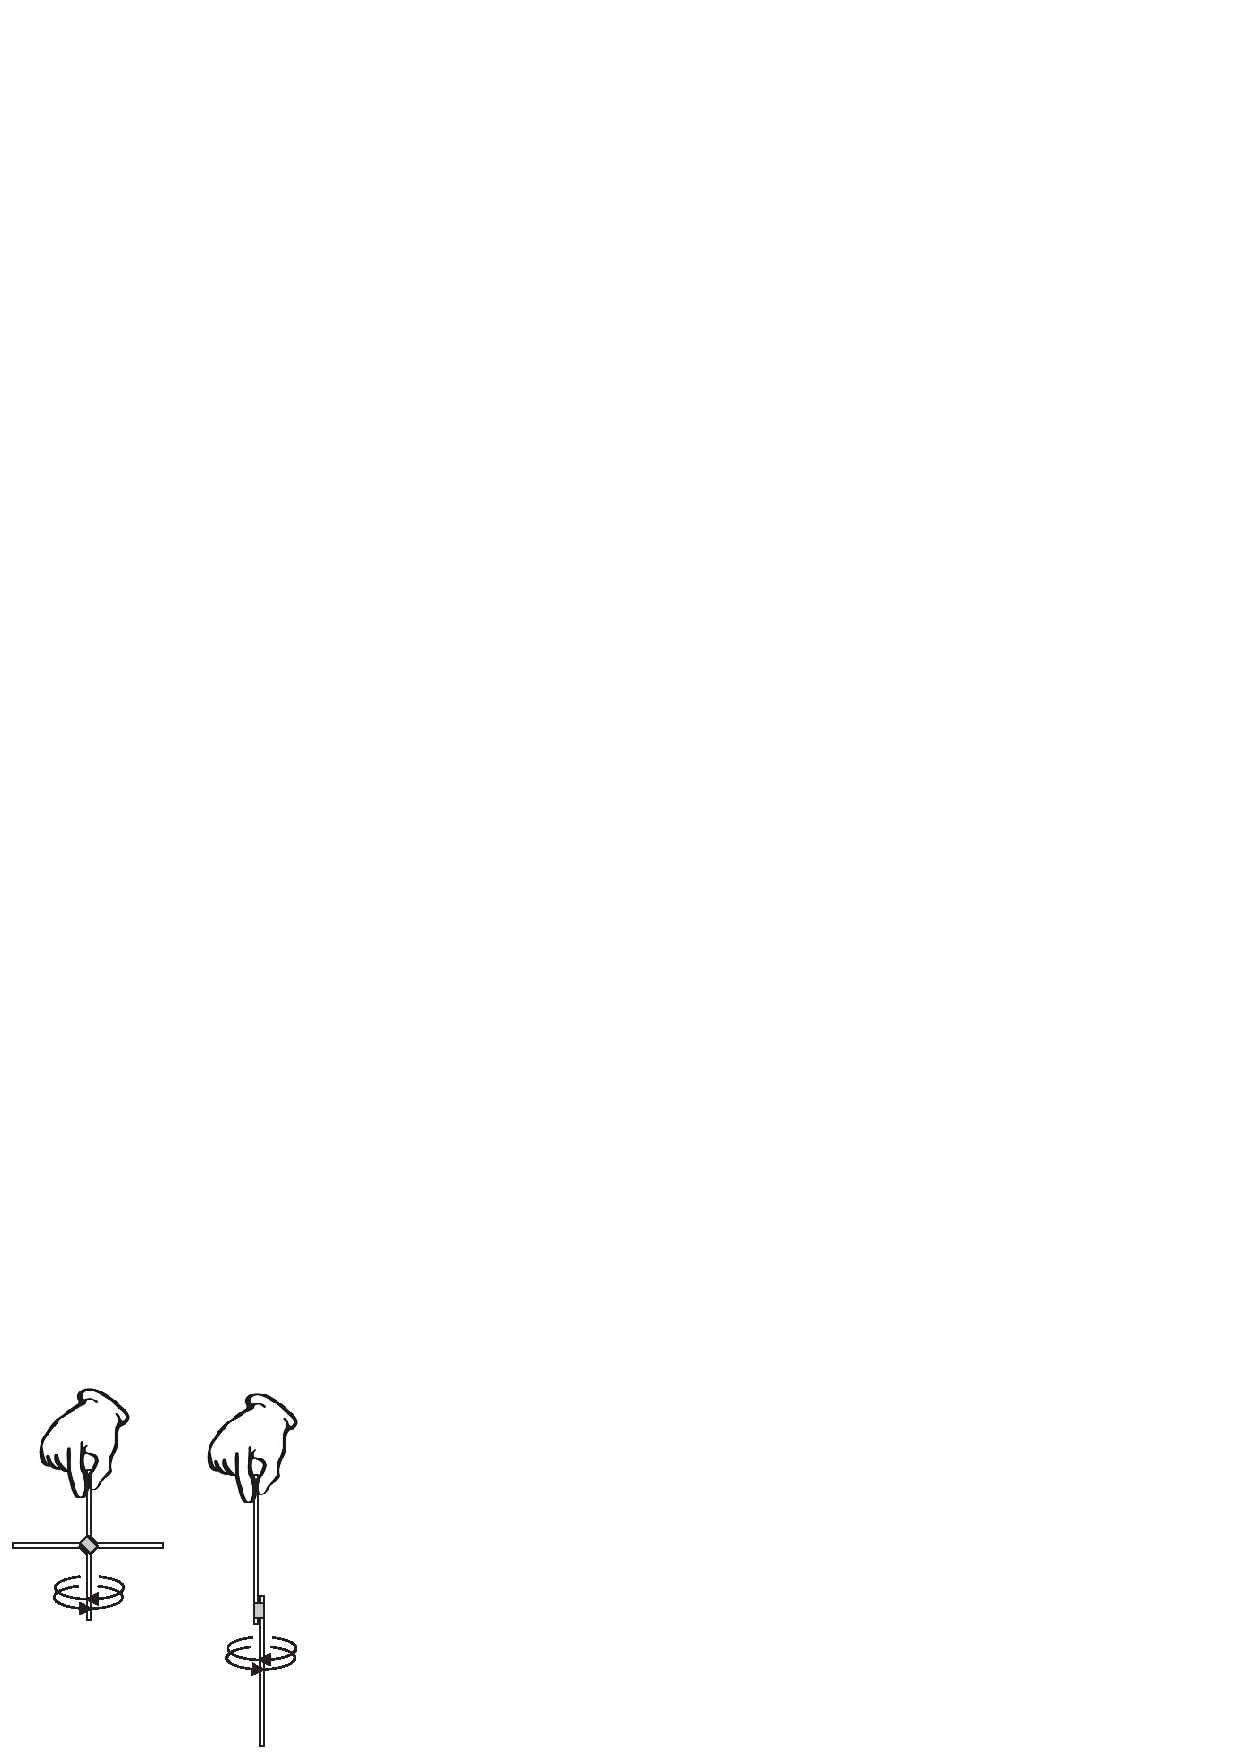
\includegraphics[width=0.26\textwidth]{moment_inertia_feel/stick_pics2.pdf}
\end{wrapfigure}

%\hspace{0.5in}
\phantom{indent05}
\textit{Prediction:}
% This is just about the weirdest Latex bug I've ever seen!
% In the line above, when I use \hspace, the right margin gets screwed up for the remainder of the page.
% So I replaced it with phantom space, and now it works fine.
% The weirdest thing is that it worked fine with hspace prior to January 2021!  --Matt
% As far as I can tell, wrapfig wasn't updated.  There must be a bug in Latex itself.
% I also used the phantom space a couple times below, to make the left indents align.
\answerspace{0.2in}

Now try it.  Does one feel harder to start spinning?  (If yes, which one?)

%\hspace{0.5in}
\phantom{indent05}\textit{Experiment:}
\answerspace{0.2in}

3.  Which pair of sticks ``feels heavier'' when you spin it?
\answerspace{0.3in}

The effect you feel is that each pair of sticks has a different \textit{moment of inertia}, which tells you how hard it is to make an object spin.  
\begin{itemize}[nosep]
\item An object's moment of inertia depends on how its mass is distributed.  It is larger when the mass is further away from the axis of rotation.  That's why the cross is harder to spin, even though both pairs of sticks have the same mass.

\item The moment of inertia \textit{also depends} on mass: you would feel the difference if you tried to spin two things of the same shape but different masses.  That's why the crossed sticks ``feel heavier'' when you spin them.  
\end{itemize}
4. For a quick, qualitative explanation of what \textit{mass} means, you might say something like:

%\hspace{0.5in}
\phantom{indent05}\textit{``Mass tells you how much an object resists accelerating when you apply a force.''}

Write a sentence analogous to the one above, using the terms \textit{moment of inertia}, \textit{angular acceleration}, and \textit{torque}.
\answerspace{0.3in}




